\chapter{CUDA Ballotting intrinsic Stream Compaction}
\label{ch:stream_compaction}

\lettrine[lines=3,lhang=0.33,lraise=0,loversize=0.15]{A}{n} efficient implementation of stream compaction on SIMD processors beased on \textit{bellotting} instructions is presented here.
This work is based on the followings works \cite{Billetter} and \cite{Hughes}.
\section{Introduction}
Stream compaction/reduction/scan is commonly referred as the operation of removing unwanted elements in a collection (see Figure \ref{fig:stream_compaction}). More formally, imagine we have a list of element \(A_{0...N}\) of N elements and a predicate \(p : A \to\left \{ True,False\right \} \) that bisects \(A\) in wanted and unwanted elements (ones that satisfy the predicates \(p\) and ones that don't). The stream compaction of \(A\) under \(p\) is an array \(B=\left\{x \in A | p(x) = True\right\}\). Sometimes is it enough to return \(B_{0\ldots N}\) s.t. all valid (suppose \(M \leq N\)) elements are grouped at the first \(M\) position of \(B\). 
A more general  and rigorous  definition  of prefix sum  is the following: given an associative operator \(\Diamond\), a vector \(V_{0\ldots N}\) of \(N\) elements and an identity element \(I\), the scan operation returns a vector 
\[P=\left\{I,v_0,(v_0 \Diamond v_1),(v_0 \Diamond v_1 \Diamond v_2),\ldots,(v_0\Diamond v_1 \Diamond \ldots \Diamond v_{n-2})\right\}\].

Stream reduction is a key building block in several important algorithm especially in the field of parallel programming where is not uncommon to have large and sparse data structure to process (for instance in the parallel breadth tree traversing, ray tracing problems, etc.). Sparsity can often be the cause of performance degradation of the overall parallel algorithm and it is often the cause of load imbalance/communication imbalance.
\begin{figure}
	\begin{center}
		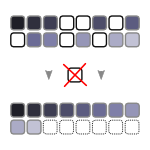
\includegraphics[width=5cm]{./images/stream_compaction/stream_compaction}
		\caption{Stream Compaction consists in removing all the elements for which the predicate is not satisfied. In this case the predicate is: \textit{color $\ne$ white}.}
		\label{fig:stream_compaction}
	\end{center}
\end{figure}

As an example, stream  compacting with the predicate \(p(x) = x >0 \) the following  array of twelve integers \(A=\left\{1,0,0,0,4,3,2,0,6,8,9,0\right\}\) would produce \(B=\left\{1,4,3,2,6,8,9\right\}\).

\subsection{Serial Algorithm}
Serial implementation in a single thread is straightforward:
 \lstset{language=C++,
	caption=Naive Serial Stream Compaction Algorithm,
	label={code:serialstreamcompaction}, 
	basicstyle=\ttfamily,
	keywordstyle=\color{blue}\ttfamily,
	stringstyle=\color{red}\ttfamily,
	commentstyle=\color{green}\ttfamily,
}
\begin{lstlisting}
template <typename T>
void serialCompact(T* input, T*output, uint length,bool (*predicate)(T)){
	uint j=0;
	for(uint i=0;i<length;i++)
		if(predicate(input[i])){
			output[j] = input[i];
			j++;
		}
}	
\end{lstlisting}
Elements satisfying the predicate are pushed into an output buffer. It can be easily implemented as a one line filter operation using the \texttt{copy\_it} operation in \texttt{C++}.

\subsection{Parallel Algorithm}
\label{sec:stream_compaction_parallel}
The parallel implementation is more challenging and the most effective parallel implementations produced so far (Thrust\cite{Thrust}, Chag:pp \cite{Billetter:2009}) are mainly based on the computation of the so called (exclusive or inclusive prefix sum). The exclusive prefix sum on a vector \(V_{0\ldots N}\) with validity test \(p\) consist in producing a vector \(S_{0\ldots N}\) s.t. \(S_0 = 0\) and \(S_i=k\) where k is the number of valid element strictly preceding (or up to the element \(i\) in case of inclusive prefix sum) the element of \(i\). Inclusive prefix sum can be obtained from exclusive using the following: let \(A=\left\{0,a_1,\ldots,a_{n-1}\right\}\) the vector of elements and \(E=\left\{0,e_1,\ldots,e_{n-1}\right\}\) its exclusive prefix sum then \(I=\left\{e_1,e_2\ldots, e_{n-1}+p(a_{n-1}) \right\}\) is the corresponding inclusive prefix sum.

Suppose \(P\) is the number of processor and \(N, N>P \)is the size of the vector. The input stream is divided in sub-streams  of size of size \(S\). The parallel algorithm is divided in three distinct phases:

\begin{enumerate}
	\item Each processor \(p_i\) count independently the number of valid elements in its sub-stream and save this value in \(procCount[p_i]\)
	\item A prefix sum operation is performed on the sub-array \(procCount\) producing the vector \(procOffset_{0\ldots P}\)
	\item Each processor can independently from the others flush out its valid elements in the correct location (at the correct offset) \(output[procOffset[p_i]+currentValidElm]\)
\end{enumerate}
 \lstset{language=C++,
	caption=Naive Serial Stream Compaction Algorithm,
	label={code:serialstreamcompaction}, 
	basicstyle=\ttfamily,
	keywordstyle=\color{blue}\ttfamily,
	stringstyle=\color{red}\ttfamily,
	commentstyle=\color{green}\ttfamily,
	backgroundcolor = \color{light-gray}
}
\begin{lstlisting}
//phase1
for each processor p in parallel
	int count=0;
	for(int i=0;i<S;i++)
		if(valid(input_p[i])
			count++;

procCount[p]=count;

//phase 2
procOffset = prefixSum(procCount)

//phase3
for each processor p in parallel
	int j=0;
	for(int i=0;i<S;i++)
		if(valid(input_p[i]){
			output[procOffset[p] + j ]
			j++;
		}
}	
\end{lstlisting}

It is worth to note that phase $2$ can also be carried out in parallel and that its implementation on SIMT hardware is not straightforward and is not discussed here. We will then use available implementation as the one shipped with the thrust library. In CUDA usually this phase load is negligible with the respect to the other two as the number of processor $P$ is usually several order of magnitude smaller than $N$.

\section{SIMT/Ballotting instruction Implementation}
\subsection{CUDA Hardware}
GPUs hardware is made of a number of order of tens streaming multiprocessors (SMM), that roughly speaking are SIMD processors made up of streaming processor (the SIMD lanes, SP). For instance the newest (2017) Volta Architecture introduced by NVIDIA counts 84 SMM and 64 SP per SMM, for a total of 5376 cores. See Figure \ref{fig:volta_sm} and \ref{fig:volta_architecture}.
SMM execute kernels in a SIMD fashion at group of 32 threads (a warp) that executes the same instructions in a synchronized manner. SMM are not scalar processor, and hence, using the parallel approach described in Section \ref{sec:stream_compaction_parallel} where each SMM is considered as a single scalar processor \(p\) would result in poor performance due to the large number of idle lanes lanes \( 84*(64-1)=5376-84\).
In this implementation each SMM is fully used to perform the block counting of valid elements and to finally compact the input.
\begin{figure}
	\begin{center}
		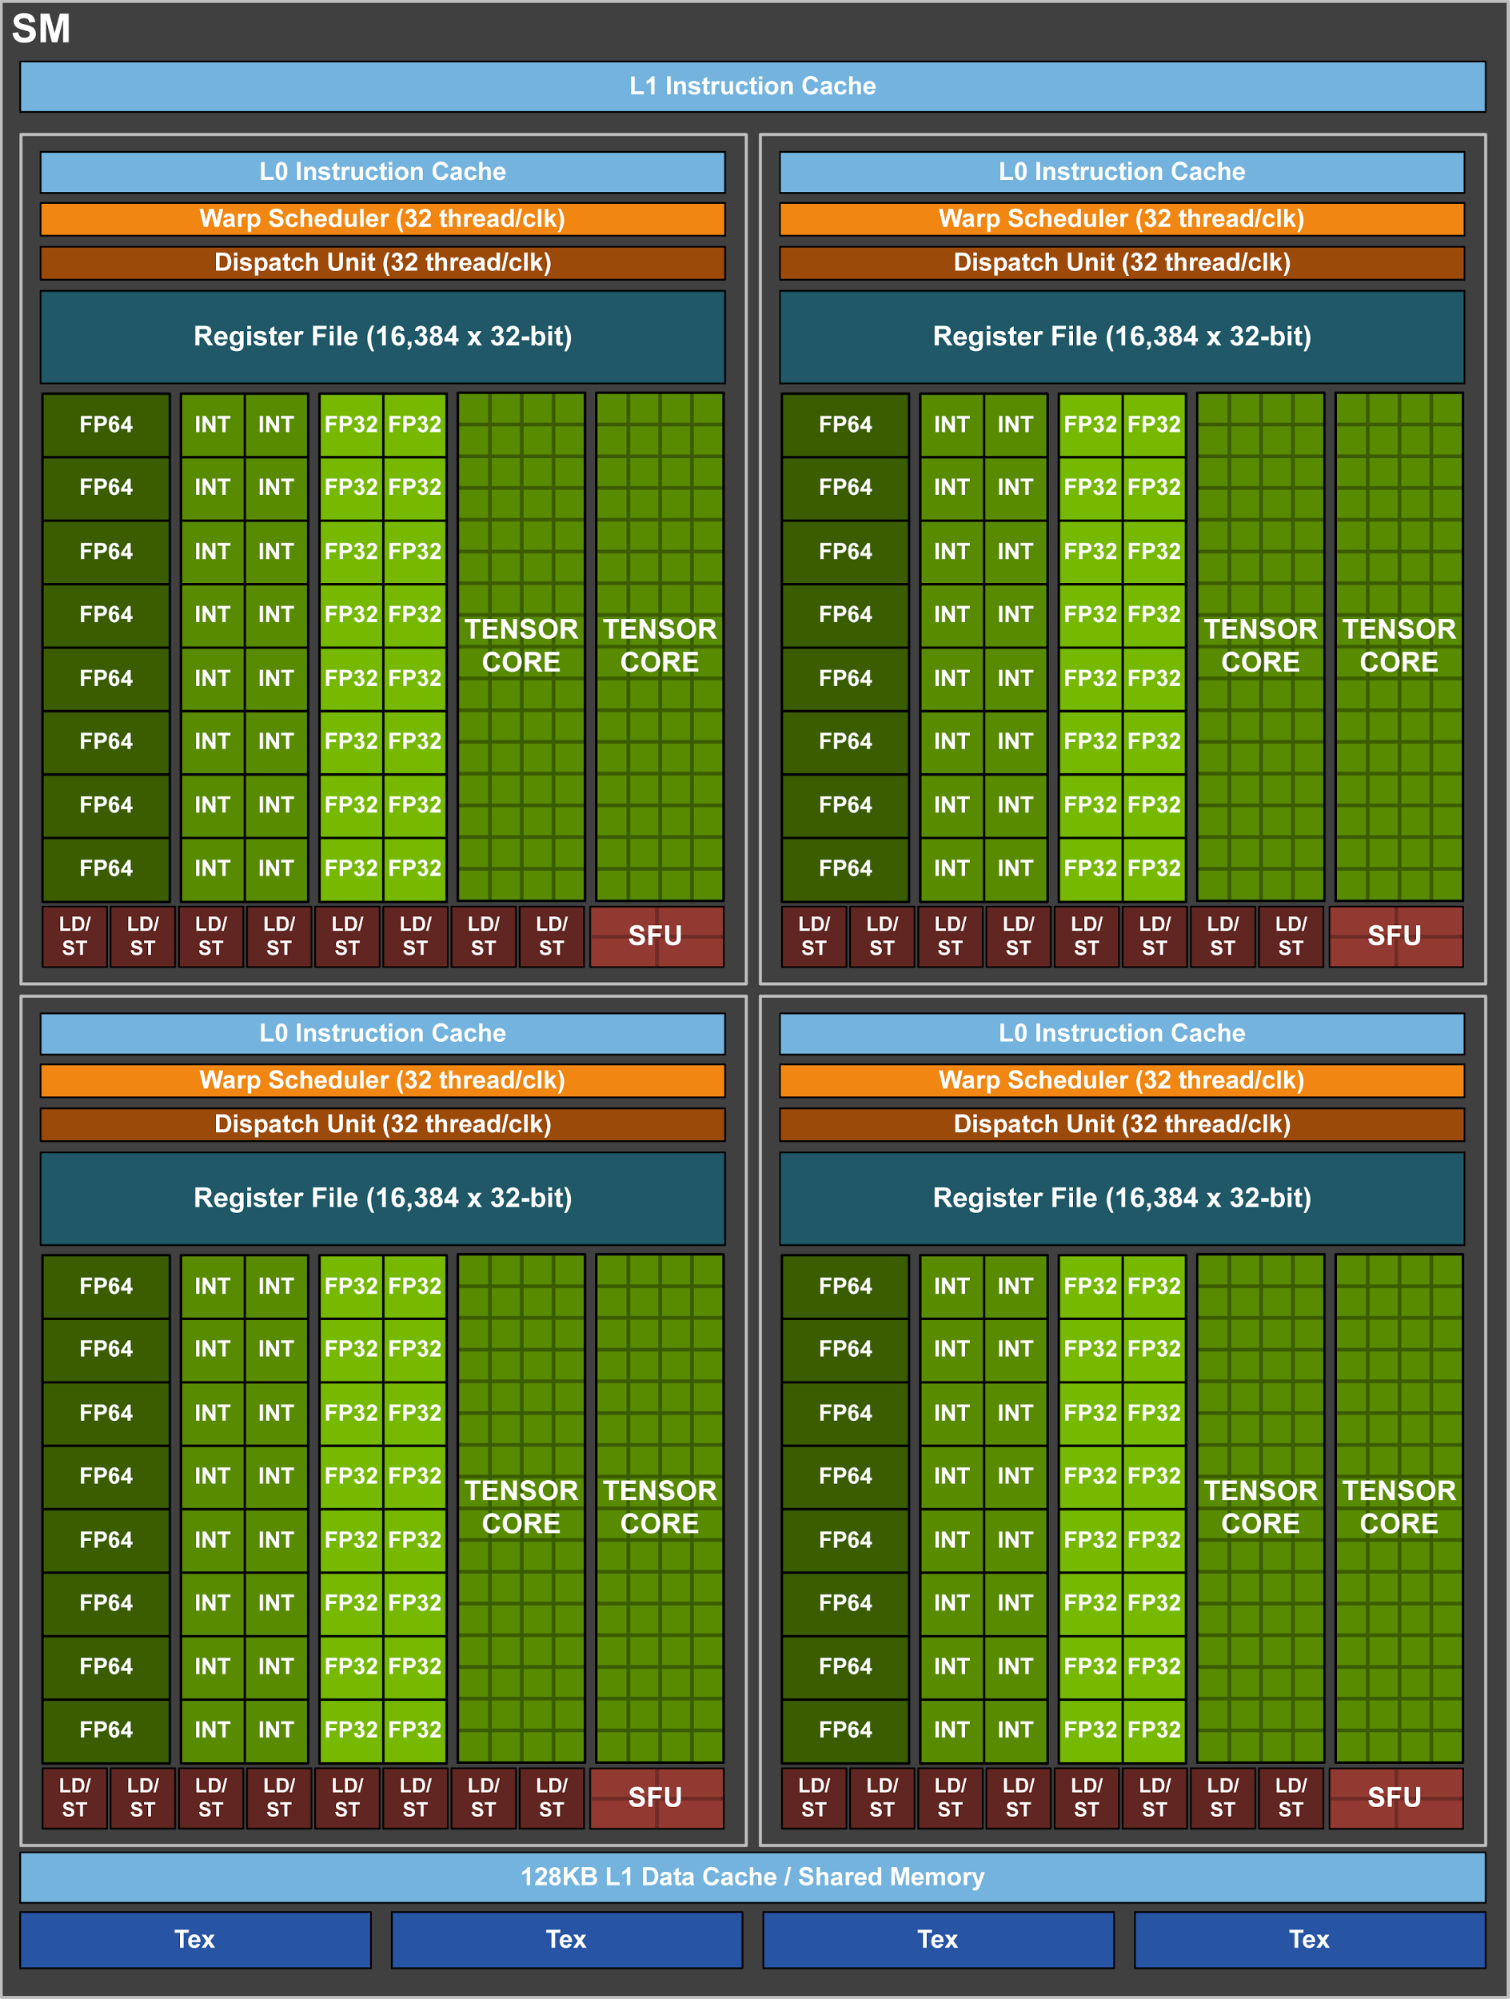
\includegraphics[width=6cm]{./images/stream_compaction/volta_sm}
		\caption{NVIDIA GPU Volta SM Architecture.}
		\label{fig:volta_sm}
	\end{center}
\end{figure}

\begin{figure}
	\begin{center}
		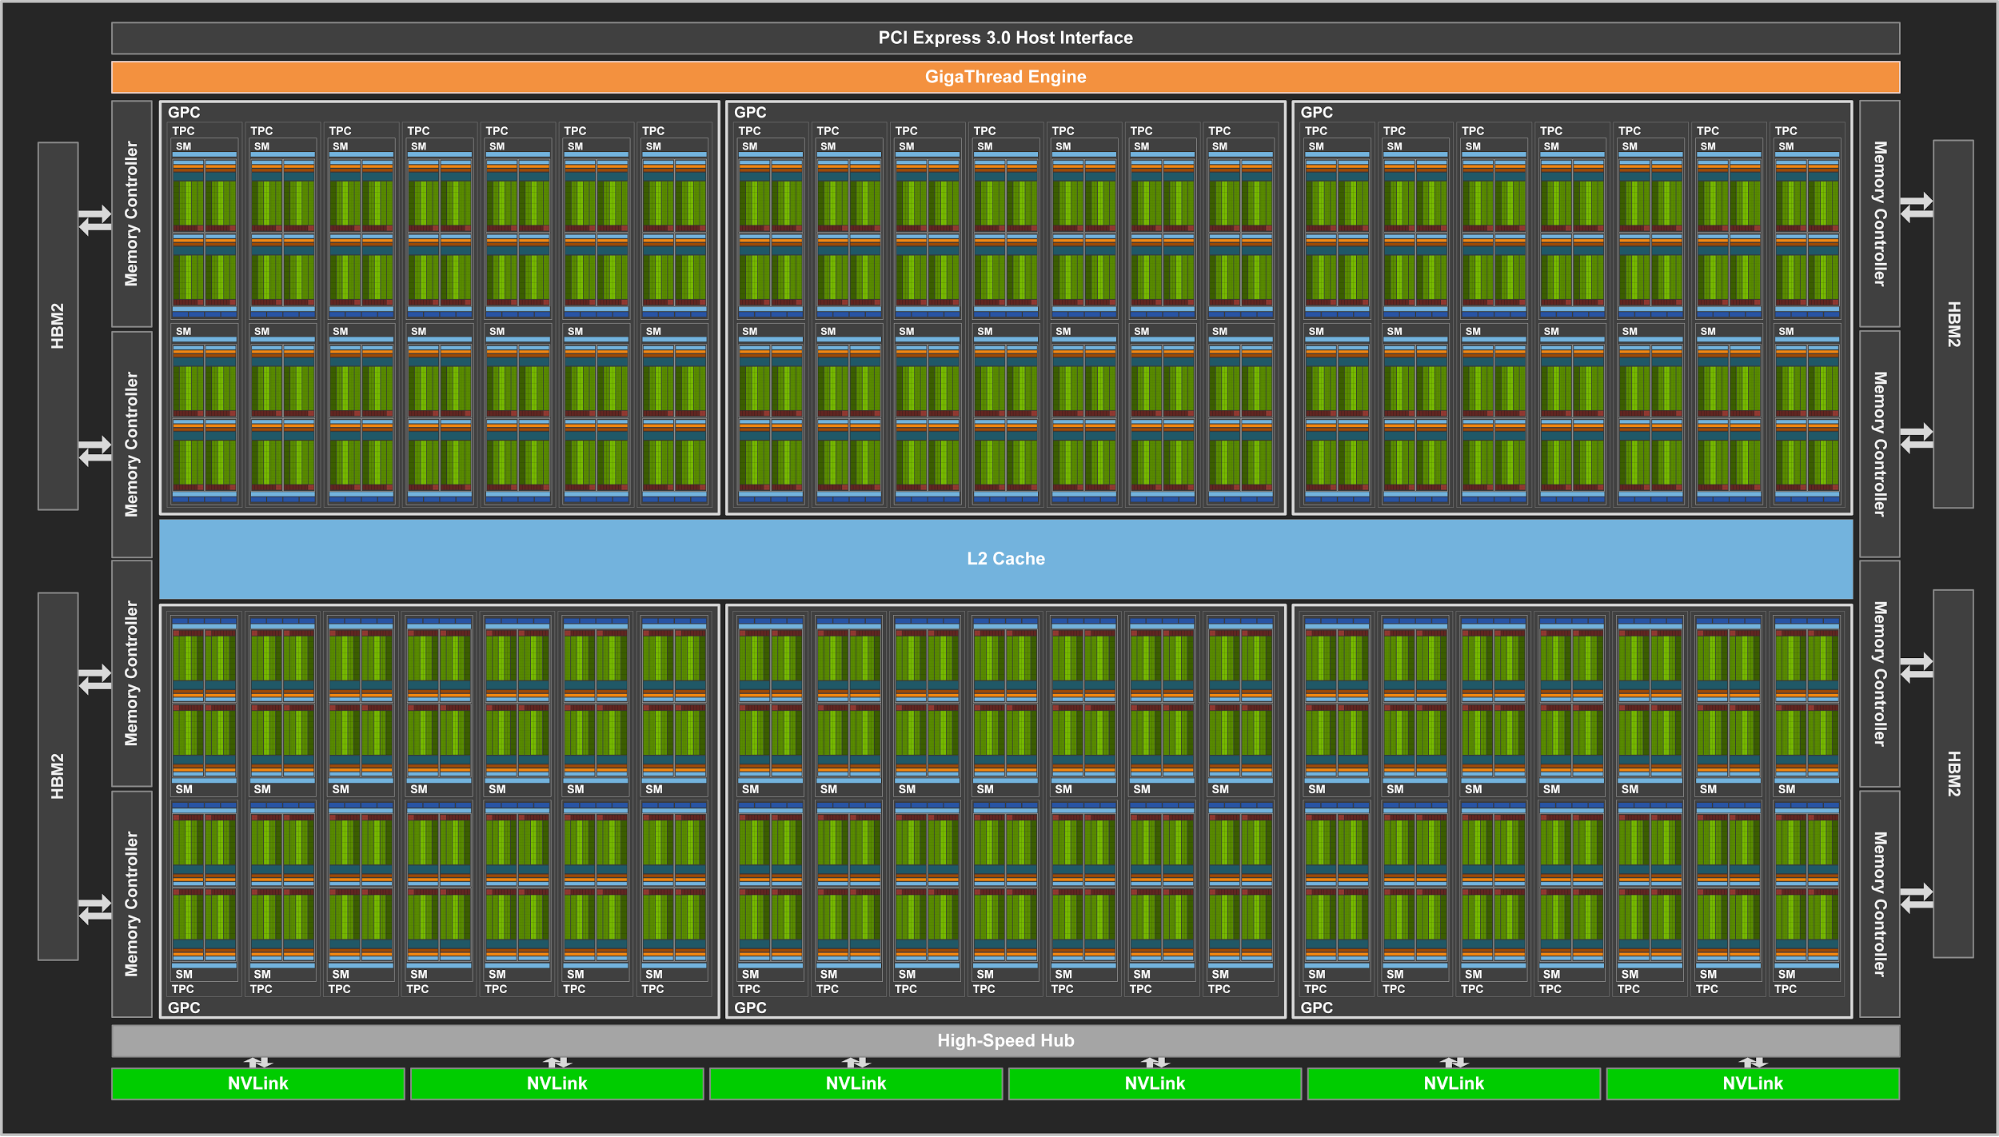
\includegraphics[width=1.0\textwidth]{./images/stream_compaction/volta_architecture}
		\caption{ Volta GV100 Full GPU with 84 SM Units.}
		\label{fig:volta_architecture}
	\end{center}
\end{figure}

\subsection{Phase $1$}
The  pseudocode \ref{code:phase1} shows how block counting can be performed on a SIMT hardware effectively using all computing lanes.
 \lstset{language=C++,
	caption=Stream Compaction phase $1$ on SIMT processor,
	label={code:phase1}, 
	basicstyle=\ttfamily,
	keywordstyle=\color{blue}\ttfamily,
	stringstyle=\color{red}\ttfamily,
	commentstyle=\color{green}\ttfamily,
	backgroundcolor = \color{light-gray}
}
\begin{lstlisting}
//input is a SMM private vector containing the portion of the //original input to be processed by the processor
for each SMM processor  p in parallel
	lanesCount[0]=0;
	...
	lanesCount[32]=0;
for(int i=0;i&amp;lt;S;i+=32)
	for each SIMD lane s in parallel
		if(predicate[input[i+s])
			lanesCount[s]++;

procCount[p] = reduce(+,lanesCount);	
\end{lstlisting}

With the introduction of the intrinsic function \texttt{\_\_syncthreads\_count(predicate)} this phase is both easier (respect to the pesudocode above) to implement and result in a more efficient and faster execution (since there is specialized transistors for executing it). This instruction synchronizes threads at block level and take an integer as predicate. It returns to \textbf{ALL thread of the block} the number of non-zero predicates passed to it by all threads of the block.
Suppose for instance that our kernel is executed only by one block made up of four threads and that each thread is calling \texttt{\_\_syncthreads\_count()} as shown in listing \ref{code:synch_call}:

 \lstset{language=C++,
	caption=\texttt{\_\_syncthreads\_count() calls from threads within a block. $1$ and $0$ represents predicate expressions. },
	label={code:synch_call}, 
	basicstyle=\ttfamily,
	keywordstyle=\color{blue}\ttfamily,
	stringstyle=\color{red}\ttfamily,
	commentstyle=\color{green}\ttfamily,
	backgroundcolor = \color{light-gray}
}
\begin{lstlisting}
//thread0
int BC=__syncthreads_count(1)
//thread1
int BC=__syncthreads_count(0)
//thread2
int BC=__syncthreads_count(1)
//thread3
int BC=__syncthreads_count(0)
\end{lstlisting}
then each thread \(t_i\) will own its private copy of the \(BC\) variable containing the value $2$.
This kind of operation is exactly what is needed in order to count the number of valid elements per block.
The previous approach can be summarized as shown in listing \ref{code:phase1simt}.
 \lstset{language=C++,
	caption=\texttt{Phase 1 implemented using ballotting intrinsic built-in functions.},
	label={code:phase1simt}, 
	basicstyle=\ttfamily,
	keywordstyle=\color{blue}\ttfamily,
	stringstyle=\color{red}\ttfamily,
	commentstyle=\color{green}\ttfamily,
	backgroundcolor = \color{light-gray}
}
\begin{lstlisting}
template <typename T,typename Predicate>
__global__ void computeBlockCounts(T* d_input,int length,int*d_BlockCounts,Predicate predicate){

int idx = threadIdx.x + blockIdx.x*blockDim.x;
if(idx < length){
	int pred = predicate(d_input[idx]);
	int BC=__syncthreads_count(pred);
	if(threadIdx.x==0)
		d_BlockCounts[blockIdx.x]=BC;
}
\end{lstlisting}

\subsection{Phase 2}
Output of Phase $1$ is a count of valid elements per block. 
Phase $2$ takes care of computing a prefix-sum among the block counters, which number is much smaller than the original input array.
For the sake of brevity and since it does not affect the overall performance because this phase is not an hot-spot for the algorithm,\texttt{Thrust} prefix sum is employed here in order to produce a vector of offsets. Offset $i$ indicates how many valid elements will be pushed by blocks $j < i$, thus actually indicating what is the block's $i$ writing index in the output array.
Listing \ref{code:phase1_simt} shows how to perform a prefix-sum on blocks's counter, output of phase $1$.
 \lstset{language=C++,
	caption=\texttt{Phase 2 implemented using a scan operation in \texttt{Thrust}.},
	label={code:phase1_simt}, 
	basicstyle=\ttfamily,
	keywordstyle=\color{blue}\ttfamily,
	stringstyle=\color{red}\ttfamily,
	commentstyle=\color{green}\ttfamily,
	backgroundcolor = \color{light-gray}
}
\begin{lstlisting}
//prefix sum thrust call
thrust::exclusive_scan(blockCounters, blockCounters + numBlocks, blockOffsets);
\end{lstlisting}

\subsection{Phase $3$}
Phase 3

The most elaborate part of the algorithm takes as input the \textit{to be compacted} stream, and the block offsets computed during the previous phases outputting the compacted stream.
It is based on the intra warp voting function \texttt{\_\_ballot()}, ans \texttt{\_\_popc()} procedure and a bit manipulation. 

The \verb|unsigned int __ballot(int predicate);| function.
evaluates \verb|predicate| for all threads of the warp and 
returns an integer whose $i^{th}$ bit is set if and only if \verb|predicate| evaluates to \textbf{non-zero} for the $i^{th}$ thread of the warp.

\verb|__popc(int number)| function returns the number of set bits in its parameter.

It is worth to note that the underlying maching has to support a wordsize which size is not smaller that the size of the warp. This could be a problem is the warp-size will be increased in the future releases of CUDA (even if this is unlikely to happen).

As shown in \ref{code:phase3_1}, this phase starts computing a per warp offset (intra warp prefix sum) offset. This means that the offset computed for the last thread of the warp is the warp's number of valid elements. Each thread  store its offset in a register while warp's valid elements are stored in a \textbf{shared memory} buffer (\verb|warpTotal[warpIDX]|). 
 \lstset{language=C++,
	caption=\texttt{Intra warp prefix-sum using ballotting intrisic},
	label={code:phase3_1}, 
	basicstyle=\ttfamily,
	keywordstyle=\color{blue}\ttfamily,
	stringstyle=\color{red}\ttfamily,
	commentstyle=\color{green}\ttfamily,
	backgroundcolor = \color{light-gray}
}
\begin{lstlisting}
int pred= predicate(threadInput);
int w_i = threadIdx.x/warpSize; //warp index
int w_l = idx % warpSize;//thread index within a warp (warp lane)
int t_m = INT_MAX >> (warpSize-w_l-1);
int b = __ballot(pred) & t_m;
int t_u = __popc(b);
//last thread of the warp stores in Shared Memory
if(w_l==warpSize-1)
	warpTotals[w_i]=t_u + pred;
__syncthreads();
\end{lstlisting}
where \verb|w_i| is the warp index within the block,\verb|w_l| is the thread index within the warp and \verb|t_m| is the thread mask, i.e. a number the only bits set are the ones with index less then \verb|w_l|. \verb|b| contains only set bits corresponding to the validity of predicated of threads of lower index. \verb|__popc(int number)| is then used to retrieve the number of set bits. \verb|t_u| is the warp offset of thread \verb|w_l|.
A block memory fence is necessary in order to ensure correctness for future access to the shared mermory array \verb|warpTotals|.

At this point  intra block scan operation is performed on \(warpOffset\) in order to compute a per-block offset. Assuming \( warpsize >= \frac{blocksize}{warpsize} \) i.e. the number of warps in a block does not exceed the size of a single warp, this operation can be performed by a single warp. This scan operation is performed in \(log_2(warpsize)\) steps because we are summing up numbers which max value is $warpsize$ (each warp cannot perform more write than its number of threads). Usually in CUDA this number is $32$ hence bit scan performed in \(log_2(32)=5\) steps.

As shown in the listing \ref{code:phase3_02}, a intra block scan operation is now performed on the the \(warpOffset\) vector in order to compute a per-block offset. It can be performed by just one warp (assuming the number of warps does not exceed the size of a warp (\( warpsize >= \frac{blocksize}{warpsize} \)). The scan operation is performed in \(log2(warpsize)\) steps because we are summing up numbers which max value is warpsize (each warp cannot perform more writes than the number of threads it is composed of). Usually in CUDA this number is $32$ hence bit scan performed in $5$ steps.
 \lstset{language=C++,
	caption=\texttt{Intra warp prefix-sum using ballotting intrisic},
	label={code:phase3_02}, 
	basicstyle=\ttfamily,
	keywordstyle=\color{blue}\ttfamily,
	stringstyle=\color{red}\ttfamily,
	commentstyle=\color{green}\ttfamily,
	backgroundcolor = \color{light-gray}
}
\begin{lstlisting}
if(w_i==0 && w_l<blockDim.x/warpSize){
	int w_i_u=0;
	for(int j=0;j<log2(warpsize);j++){
		int b_j =__ballot( warpTotals[w_l] & pow2i(j) );
		w_i_u += (__popc(b_j & t_m)  ) << j;
	}
	warpTotals[w_l]=w_i_u;
}
\end{lstlisting}
where \(b_j\) is a number in which each bit is one if and only if the \(j^{th}\) bit of the \(j^{th}\) per-warp counter  is one.
Each warp then  mask only the bits \(i'< i\) (of the warps before it)
and finally sum them up, effectively completing the prefix sum operation.


Knowing the \textit{warp}, \textit{block}, and \textit{grid offsets} is possible to flush out the valid elements from the input array at the correct locations in the output array. If the current thread is managing a valid element then if flush it out at the following location: 
$	output[t_u+warpTotals[w\_i]+blocksOffset[blockIdx.x]]= input[idx];$
which reads as: (thread's offset within its warp) + (thread's warp offset within the block) + (thread's block offset within the grid).


As an example lets suppose that a block of 4 warps produces the following \verb|warpTotals|:

\begin{verbatim}
warpTotals[0] = 16 = 1 0 0 0 0 
warpTotals[1] = 18 = 1 0 0 1 0
warpTotals[2] = 17 = 1 0 0 0 1
warpTotals[3] = 13 = 0 1 1 0 1
\end{verbatim}
Note that warp $0$ always produces zero as output because \verb|t_m = 0 >= (b_j & t_m) =0|.

\begin{description}
\item[Step 0]\hfill \\
	\(b_0\) = \verb|__ballot( warpTotals[w_l] & pow2i(0) )| = 12 (column zero)\\
	\(w_1\) = \verb|__popc(12 & 1) << 0|$ = 0 << 0 = 0$\\
	\(w_2\)= \verb|__popc(12 & 3) << 0| $= 0 << 0  = 0$\\
	\(w_3\)= \verb|__popc(12 & 7) << 0| $= 1 << 0  = 1$\\
	
	\item[Step 1]\hfill \\
	\(b_0\) = \verb|__ballot( warpTotals[w_l] & pow2i(1) )| = 2 (column one)\\
	\(w_1\) = \verb|__popc(2 & 1) << 1|$ = 0 << 1 = 0$\\
	\(w_2\)= \verb|__popc(2 & 3) << 1| $= 0 << 1  = 2$\\
	\(w_3\)= \verb|__popc(2 & 7) << 1| $= 1 << 1  = 2$\\
	
	
	\item[Step 2]\hfill \\
	\(b_0\) = \verb|__ballot( warpTotals[w_l] & pow2i(2) )| = 8 (column two)\\
	\(w_1\) = \verb|__popc(8 & 1) << 2|$ = 0 << 2 = 0$\\
	\(w_2\)= \verb|__popc(8 & 3) << 2| $= 0 << 2 = 0$\\
	\(w_3\)= \verb|__popc(8 & 7) << 2| $= 1 << 2  = 0$\\
	
		\item[Step 3]\hfill \\
	\(b_0\) = \verb|__ballot( warpTotals[w_l] & pow2i(2) )| = 8 (column three)\\
	\(w_1\) = \verb|__popc(8 & 1) << 3|$ = 0 << 3 = 0$\\
	\(w_2\)= \verb|__popc(8 & 3) << 3| $= 0 << 3  = 0$\\
	\(w_3\)= \verb|__popc(8 & 7) << 3| $= 1 << 3  = 0$\\
	
	
	\item[Step 4]\hfill \\
	\(b_0\) = \verb|__ballot( warpTotals[w_l] & pow2i(4) )| = 7 (column four)\\
	\(w_1\) = \verb|__popc(7 & 1) << 4|$ = 16 << 4 =0$\\
	\(w_2\)= \verb|__popc(7 & 3) << 4| $= 36 << 4 =0$\\
	\(w_3\)= \verb|__popc(7 & 7) << 4| $= 48 << 4 =1$\\
	
\end{description}

The final result for each warp is simply the sum of the $w_{i\,u}$ at all steps\\
\(w_0 = 0 + 0 + 0 + 0 + 0 = 0\)\\
\(w_1 = 0 + 0 + 0 + 0 + 16 = 16\)\\
\(w_2 = 0 + 2 + 0 + 0 + 36 = 38 = 16+18=34\)\\
\(w_3 = 1 + 2 + 0 + 0 + 48 = 51 = 16+18+17=51\)\\


%\section{Performance Tests}

%TODO